\documentclass[runningheads]{llncs}
\usepackage{hyperref}
\usepackage[T1]{fontenc}
\usepackage{graphicx}
\usepackage[spanish]{babel}
\usepackage{color}
\renewcommand\UrlFont{\color{blue}\rmfamily}
\urlstyle{rm}

\begin{document}

\title{Proyecto de IA - Simulación \\
        Major League Baseball}

\author{Alejandro Álvarez Lamazares \\
        Marian S. Álvarez Suri \\
        Carlos A. Bresó Sotto
        }

\authorrunning{A. Álvarez, M. S. Álvarez, C. A. Bresó}

\institute{Facultad de Matemática y Computación. Universidad de La Habana}

\maketitle

\begin{abstract}
    Este reporte describe el desarrollo y resultados del proyecto de inteligencia artificial y simulación aplicado a la Major League Baseball (MLB). En particular, se realizó una simulación de los partidos de la temporada 2022 de la MLB, utilizando elementos de IA como algoritmos de búsqueda, conocimiento y procesamiento de lenguaje natural. En la simulación, los agentes fueron tratados desde el enfoque de Beliefs - Desires - Intentions (BDI), lo que permitió modelar de manera más realista las decisiones estratégicas y comportamientos de los managers.
\end{abstract}

\section{Introducción}
    El objetivo de este proyecto es simular los juegos de la temporada 2022 de la Major League Baseball (MLB) \cite{mlb} utilizando técnicas avanzadas de inteligencia artificial y simulación. La simulación permite observar cómo diferentes estrategias pueden afectar el resultado de un juego, proporcionando una herramienta valiosa para entrenadores, analistas y aficionados al béisbol.
    
    Nuestra propuesta de solución incluye un algoritmo genético para optimizar la selección del lineup, asegurando que los jugadores más adecuados estén en el campo de juego. Además, el manager virtual toma decisiones estratégicas basadas en un sistema experto, que evalúa las estadísticas y situaciones del juego en tiempo real. Finalmente, hemos implementado un comentarista virtual utilizando procesamiento de lenguaje natural con la IA Gemini \cite{gemini}.


\section{Datos y Preprocesamiento}
    Los datos utilizados en el proyecto incluyen estadísticas de jugadores y equipos de la temporada 2022 de la MLB, así como información sobre los partidos y resultados de dicho año. Los datos se obtuvieron de la página BaseballSavant \cite{baseballsavant} y mediante el uso de la librería statsapi \cite{statsapi}. El preprocesamiento de los datos incluyó su limpieza y transformación para que fueran compatibles con los algoritmos utilizados en el proyecto.

\section{Simulación del Juego}
    La fase de simulación del juego es una parte crucial del proyecto, donde se modelan las dinámicas y reglas del béisbol para replicar los partidos de la temporada 2022 de la MLB. En esta fase, se utiliza la estructura de Beliefs-Desires-Intentions (BDI) para crear los agentes, que en este caso son los managers de los equipos.

    \subsection{Calendario de enfrentamientos}
        El calendario de enfrentamientos se generó de forma aleatoria, de acuerdo con el formato de la temporada regular de la MLB. Cada equipo juega un total de 162 partidos, distribuidos en series de 3 o 4 partidos contra los demás equipos de su liga.

        La MLB está dividida en dos ligas: la Liga Americana (AL) y la Liga Nacional (NL), cada una de las cuales se subdivide en tres divisiones: Este, Central y Oeste. Durante la temporada regular, los equipos juegan la mayoría de sus partidos contra equipos de su propia división, así como un número significativo de partidos contra equipos de la misma liga pero de diferentes divisiones. También hay una cantidad limitada de partidos interligas, donde equipos de la AL juegan contra equipos de la NL.

        Al final de la temporada regular, los equipos con el mejor récord en cada división avanzan a la postemporada, junto con los equipos con los mejores récords restantes (wild cards). La postemporada incluye una serie de rondas eliminatorias que culminan en la Serie Mundial, donde los campeones de la AL y la NL se enfrentan para determinar el campeón de la MLB.


    \subsection{Modelo del Juego}
        El modelo del juego incluye las reglas y dinámicas del béisbol, como las posiciones de los jugadores, las acciones posibles en cada turno al bate y las situaciones de juego. El juego se divide en turnos al bate, donde un equipo intenta anotar carreras y el otro equipo intenta evitarlo. Cada turno al bate consta de una serie de lanzamientos, bateos y corridas, que pueden resultar en outs, hits, carreras o cambios de turno. 

        Para determinar el resultado de cada turno al bate, se simula el enfrentamiento entre el pitcher y el bateador en turno, teniendo en cuenta las estadísticas de ambos jugadores. Se consideran factores como la capacidad del bateador para ganar boletos a primera base y hacer hits, la habilidad del pitcher para evitarlo; así como la destreza de los jugadores que defienden para lograr outs en jugadas complejas. Además, se tienen en cuenta las situaciones de juego, como la cantidad de outs, los corredores en base, el desgaste del pitcher y el marcador actual, para determinar las decisiones estratégicas que toma el manager. 

        Las decisiones del manager surtirán efecto basadas también en las estadísticas que incumben a los jugadores, como la velocidad de los corredores, el posiscionamiento del infield defensivo y la habilidad del bateador para hacer contacto con la bola.

    \subsection{Estructura BDI para los Agentes}
        La estructura BDI es un modelo de agentes que se basa en tres componentes principales \cite{rao1995bdi}:
        \begin{itemize}
            \item \textbf{Creencias (Beliefs)}: Representan la información que el agente tiene sobre el funcionamiento del juego y el estado actual del mismo. Constituyen el conjunto de condiciones que tienen que cumplirse para aplicar cierta regla.
            \item \textbf{Deseos (Desires)}: Son los objetivos que el agente quiere alcanzar, como anotar más carreras, defender la ventaja o tomar una alternativa conservadora. A partir del estado del juego, se determina cuáles de los objetivos quieren cumplirse con mayor interés y, por tanto, qué conjunto de reglas se deben considerar.
            \item \textbf{Intenciones (Intentions)}: Son las acciones que el agente decide llevar a cabo para alcanzar sus deseos, basándose en sus creencias.
        \end{itemize}

    \subsection{Tipos de Managers}
        En la simulación, pueden existir diferentes tipos de managers, cada uno con su propio estilo y estrategia:
        \begin{itemize}
            \item \textbf{Manager Agresivo}: Toma decisiones arriesgadas para intentar obtener una ventaja significativa. Este tipo de manager puede decidir cambiar a un bateador por uno emergente o intentar robos de base en situaciones críticas.
            \item \textbf{Manager Defensivo}: Se concentra en mantener la ventaja del juego indicando acciones como vigilar al corredor en base para evitar robos.
            \item \textbf{Manager Conservador}: Prefiere tomar decisiones seguras y minimizar riesgos. Por ejemplo, puede optar por otorgar una base por bolas intensional para mantener la ventaja.
            \item \textbf{Manager Neutral}: Considera todos los posibles tipos de reglas que pueden efectuarse, siempre que estas tengan sentido.
        \end{itemize}

    \subsection{Decisiones del Manager}
        Las decisiones que puede tomar cada manager incluyen, pero no se limitan a:
        \begin{itemize}
            \item \textbf{Cambio de Pitcher}: Decidir cuándo cambiar al pitcher actual por uno del bullpen, basado en el rendimiento y la fatiga del pitcher.
            \item \textbf{Robo de Base}: Decidir cuándo intentar un robo de base, considerando la velocidad del corredor.
            \item \textbf{Bateador Emergente}: Cambiar al bateador de turno por uno emergente que no se encontraba en la alineación pero que podría representar una clara ventaja ofensiva en el actual turno al bate.
            \item \textbf{Jugada de Corrido y Bateo}: Indicar un intento de jugada de corrido y bateo basado en el contacto del bateador y en la velocidad del corredor.
            \item \textbf{Pickoff}: Indicarle al pítcher que realice lanzamientos a la base donde se encuentre el corredor si considera que existe amenaza de robo de base.
        \end{itemize}


        El conjunto de decisiones que pueden tomar nuestros agentes se basa en qué porcentaje de cada tipo de manager es. Dado un estado determinado del juego, se determina cuán agresivo, defensivo, conservador y neutral debería ser un manager para, a partir de los porcentajes determinados, incluir un conjunto de reglas a ser consideradas. De esta forma, podemos tener managers totalmente agresivos, parcialmente conservadores y defensivos, o cualquier otra combinación posible.

\section{Inteligencia Artificial}
    Los elementos de inteligencia artificial integrados permiten un mejor acercamiento a la realidad. Empleamos tres enfoques fundamentales durante las simulaciones con algoritmos de búsqueda, conocimiento y procesamiento de lenguaje natural.

    \subsection{Algoritmo de Búsqueda}

        El béisbol es un deporte que involucra una gran cantidad de variables y decisiones estratégicas. La selección del mejor lineup para un equipo es un problema complejo que requiere considerar múltiples factores, como las estadísticas de rendimiento de los jugadores, las restricciones de posicionamiento y la importancia del orden. Un \textbf{algoritmo genético} es particularmente adecuado para este problema debido a la posibilidad de explorar un amplio espacio de soluciones y encontrar lineups que maximicen el rendimiento del equipo. Basándonos en el principio de conservar los jugadores que maximicen la función de evaluación, se logra mejorar en cada iteración el resultado final y acomodar las posiciones definitivas que ocupará cada jugador. El proceso de selección del lineup implica los siguientes pasos:

        \begin{enumerate}
            \item \textbf{Inicialización}: Se genera una población inicial de posibles lineups de manera aleatoria.
            \item \textbf{Evaluación}: Cada lineup se evalúa utilizando una función de aptitud que considera factores como las estadísticas de bateo de los jugadores y la efectivadad defensiva.
            \item \textbf{Selección}: Se seleccionan los mejores lineups basados en su aptitud para formar una nueva generación. Empleamos la estrategia de selección por torneos \cite{tournamentselection} para elegir los lineups más aptos porque, a diferencia de la estrategia de selección por rueda \cite{roulettewheelselection}, permite una mayor diversidad a la hora de discernir entre soluciones muy similares.
            \item \textbf{Cruzamiento}: Se combinan pares de lineups seleccionados para crear nuevos lineups, intercambiando características entre ellos. Uno de los elementos más influyentes en nuestro problema es el mantenimiento del orden, por lo que conservamos secciones de line-up sin variación y solo intercambiamos jugadores en otras secciones.
            \item \textbf{Mutación}: Se introducen pequeñas modificaciones aleatorias en algunos lineups para mantener la diversidad genética y evitar la convergencia prematura. En cada iteración, existe cierta probabilidad de que alguno de los jugadores en los lineups sea mutado y sustituido por otro beisbolista disponible.
            \item \textbf{Iteración}: Los pasos de evaluación, selección, cruzamiento y mutación se repiten durante varias generaciones hasta que se alcanza el criterio de parada convenido, el cual depende de un tiempo determinado.
        \end{enumerate}

    \subsection{Algoritmo de Conocimiento}
        Los managers constituyen una parte fundamental en el desarrollo de un juego de béisbol. La toma de decisiones estratégicas, como cuándo cambiar al pitcher o cuándo intentar un robo de base, puede influir significativamente en el resultado del juego. Para modelar el comportamiento de los managers, utilizamos un \textbf{sistema experto} que evalúa las situaciones del juego y toma decisiones basadas en reglas predefinidas. El sistema experto se basa en un conjunto de reglas que representan el conocimiento y la experiencia de un manager real, y se utiliza para determinar las acciones más adecuadas en cada situación. Las reglas se definen en función de los deseos del manager, que son determinados a partir del estado del juego. 

    \subsection{Algoritmo de Procesamiento de Lenguaje Natural}
        El comentarista virtual es un elemento novedoso en la simulación, ya que proporciona información y análisis sobre el desarrollo del juego. Para implementar el comentarista virtual, utilizamos el \textbf{modelo de lenguaje Gemini} de OpenAI, que es capaz de generar texto coherente y relevante en función de una entrada dada. El comentarista virtual recibe información sobre el estado del juego en cada turno al bate, como el marcador actual, los jugadores en base y el número de outs, y genera comentarios que describen lo que está sucediendo.


\section{Resultados}
    Los resultados de la simulación muestran cómo diferentes decisiones estratégicas pueden influir en el resultado del juego. A continuación, se presenta un análisis de los resultados obtenidos en la simulación, comparando las métricas entre la Liga Nacional (NL) y la Liga Americana (AL):

    % Imagen
    \begin{figure}[h]
        \centering
        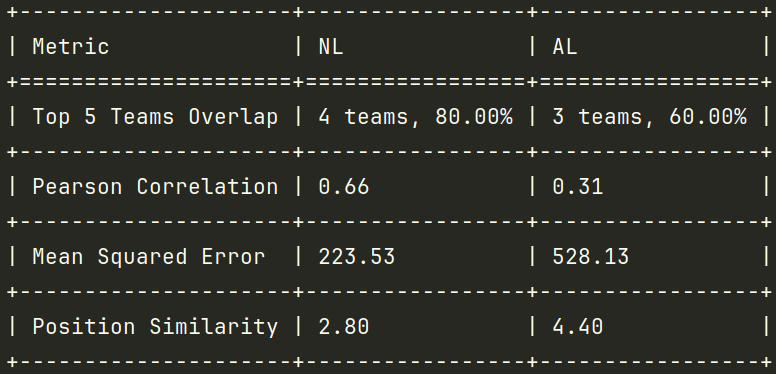
\includegraphics[width=0.8\textwidth]{metrics_table.png}
        \caption{Comparación de métricas entre la NL y la AL}
    \end{figure}

    \begin{itemize}
        \item \textbf{Top 5 Teams Overlap}: Esta métrica mide el porcentaje de coincidencia entre los cinco mejores equipos en la simulación y los resultados reales. En la NL (National League), hubo un 80.00\% de coincidencia en los cinco mejores equipos entre la simulación y los resultados reales, mientras que en la AL (American League), la coincidencia fue del 60.00\%.
        \item \textbf{Pearson Correlation}: La correlación de Pearson mide la relación lineal entre las posiciones simuladas y las posiciones reales. Un valor más cercano a 1 indica una mejor relación lineal. La correlación de Pearson entre las posiciones simuladas y las posiciones reales fue de 0.68 para la NL y 0.31 para la AL. Una correlación más alta en la NL indica una mejor relación lineal entre las posiciones simuladas y las reales en comparación con la AL \cite{pearson1895}.
        \item \textbf{Mean Squared Error (MSE)}: El MSE mide el promedio de los cuadrados de los errores, es decir, la diferencia entre los valores simulados y los valores reales. Un MSE más bajo indica predicciones más cercanas a los resultados reales. El error cuadrático medio (MSE) fue de 325.47 para la NL y 342.20 para la AL. Un MSE más bajo en la NL indica que las predicciones de la simulación fueron más cercanas a los resultados reales en comparación con la AL \cite{mse}.
        \item \textbf{Position Similarity}: Esta métrica mide la similitud entre las posiciones simuladas y las posiciones reales. Un valor más bajo indica una mayor similitud. La similitud de posiciones fue de 2.80 para la NL y 4.27 para la AL. Un valor más bajo en la NL sugiere que las posiciones simuladas estuvieron más cerca de las posiciones reales en comparación con la AL \cite{positionsimilarity}.
    \end{itemize}

    En general, los resultados indican que la simulación fue altamente precisa y efectiva para ambas ligas, sobre todo en la NL. 

\section{Conclusiones}
    El proyecto evidencia que es posible utilizar técnicas de inteligencia artificial para simular juegos de béisbol y tomar decisiones estratégicas.
    Demuestra, de igual forma, la eficacia de las estrategias de simulación evaluadas y la similitud con los juegos reales. Esto puede ser útil para entrenadores y analistas que buscan optimizar sus estrategias de juego.

\bibliographystyle{IEEEtran}
\bibliography{referencias}

\end{document}